\chapter{نرم‌افزار و الگوریتم‌های مورد استفاده}
\section{مقدمه}
در این فصل بعد از طراحی و ساخت قطعات ربات و سپس اسمبل کردن آن به بحث نرم‌افزاری پروژه می‌پردازیم. در ابتدا با چند پروتکل و تکنیک آشنا می‌شویم که در مسیر انجام دقیق پروژه از آن‌ها استفاده می‌کنیم که عبارت است از 
\lr{UART} و \lr{PWM}.
به دلیل استفاده از میکروکنترلر \lr{STM32}، تنظیمات اصلی و پایه‌های آن را در نرم‌افزار  \lr{CubeMX} انجام می‌دهیم و در ادامه در محیط  \lr{Keil} شروع به برنامه‌نویسی روی میکروکنترلر می‌کنیم. برای مرتب شدن کد سعی کردیم تا جایی که امکان دارد هر قسمت کد را جدا کرده و به صورت تابع بنویسیم. در نهایت هم با بررسی‌های فراوان، چهار حرکت اصلی ربات را بدست آوردیم.
\section{پروتکل \lr{UART}}
پروتکل‌های ارتباطی نقش مهمی را در سازماندهی ارتباطات بین دستگاه‌های مختلف بازی می‌کنند. این پروتکل ها بر اساس نیازهای هر سیستم در حالت‌های متفاوتی طراحی شده‌اند و با تعریف قوانین مشخص که در دستگاه‌های مختلف مشترک می‌باشد می‌توانند ضامن یک ارتباط موفق و پایدار در شبکه باشند.

سیستم‌های جاسازی شده، میکروکنترلرها و کامپیوترها غالباً از \lr{UART} به عنوان پروتکلی سخت افزاری برای برقراری ارتباط بین دستگاه‌های مختلف استفاده می‌کنند. در میان پروتکل‌های سخت افزاری موجود، \lr{UART} برای ارسال و دریافت داده تنها از دو سیم بهره می‌برد.

\lr{UART}
مخفف
\lr{Universal Asynchronous Receiver-Transmitter}
به معنی فرستنده و گیرنده سریال ناهمزمان جهانی است. دو سیگنال در هر \lr{UART} به صورت زیر نام گذاری می‌شود:
    \begin{figure}[!h]
    \centering
	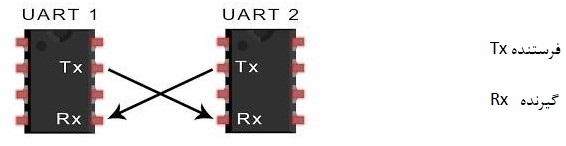
\includegraphics[height=4cm,width=15cm]{./Images/CH4/UART_1.jpg}
	\caption[سیگنال های فرستنده گیرنده \lr{UART}]{سیگنال های فرستنده گیرنده \lr{UART}}
	\label{سیگنال فرستنده و گیرنده}
	\end{figure}
	
بخش فرستنده \lr{UART} به یک باس کنترل‌کننده داده‌ها متصل شده و اطلاعات به صورت موازی به کنترل کننده ارسال می‌شود، سپس داده‌ها به صورت سریال و بیت به بیت روی خط انتقال (سیم) برای گیرنده \lr{UART} فرستاده می‌شوند. گیرنده \lr{UART} نیز داده‌های سریال را پیش از انتقال به گیرنده اصلی به صورت موازی درمی آورد.

\newpage
در‌واقع خطوط \lr{UART} یک نوع واسط ارتباطی هستند که اطلاعات را از یک دستگاه می‌گیرند و به دستگاهی دیگر انتقال می‌دهند که پروتکل \lr{UART} پین هایی منحصر به فرد را به انتقال یا دریافت داده اختصاص داده و یک پین نمی‌تواند هم خروجی و هم ورودی باشد.

    \begin{figure}[!h]
	\centering
	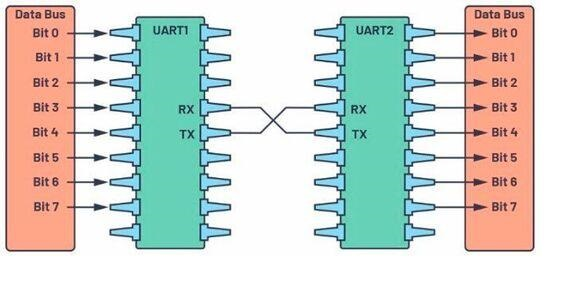
\includegraphics[height=5cm,width=9cm]{./Images/CH4/UART_2.jpg}
	\caption[رابط سریال \lr{UART}]{رابط سریال \lr{UART}}
	\label{رابط سریال}
	\end{figure}

ما برای برقراری ارتباط بین \lr{STM32} و \lr{ESP32} از پروتکل \lr{UART} استفاده می‌کنیم به این دلیل که ما از 12پایه که قابلیت \lr{PWM} دارند استفاده کردیم و تنها پروتکل موجود برای برقراری ارتباط \lr{UART} می‌باشد.

\section{تکنیک کنترلی \lr{PWM}}
\subsection{مفهوم \lr{PWM}}
در بسياري از موارد، ما نياز به كنترل ولتاژ بر روي پايه‌هاي خروجي ميكروكنترلر را داريم. مثلاً اگر بخواهيم سرعت موتور را كنترل كنيم، بايد ولتاژي كه بر روي موتور اعمال مي‌شود را كنترل كرد. در حقيقت سرعت موتور تقريباً تابع مستقيمي از ولتاژي است كه بر روي آن اعمال مي‌شود. يعني اگر ولتاژ كاريِ موتوري (ولتاژ استاندارد براي فعال سازي موتور كه بر روي بدنه‌ي آن نوشته مي‌شود) 12 ولت باشد، با اعمال ولتاژ 6 ولت روي آن، مي‌توانيد سرعت چرخش آن (\lr{rpm}\LTRfootnote{Rounds Per Minute}) را حدوداً به نصف كاهش دهيد.

\lr{PWM} مخفف \lr{pulse width modulation} یک فرآیند یا تکنیک مدولاسیون است که
در اکثر سیستم های ارتباطی برای کدگذاری دامنه سیگنال در عرض پالس یا مدت زمان سیگنال، معمولاً سیگنال حامل، به منظور انتقال استفاده می شود.

\lr{PWM} به ما این امکان را می دهد تا مدت زمان سیگنال را به صورت آنالوگ زیاد کنیم. در حالی که سیگنال در هر زمان فقط می تواند \lr{High} (معمولاً 5 ولت) یا \lr{Low} (زمین) باشد، ما می توانیم نسبت زمان \lr{High} بودن سیگنال را در مقایسه با زمانی که سیگنال \lr{Low} است در یک فاصله زمانی ثابت تغییر دهیم.

یکی از مفاهیم اساسی در فهم این که \lr{PWM} چیست، چرخه کار یا همان \lr{duty cycle} است. چرخه کار بر حسب درصد اندازه گیری می شود. چرخه کار به طور مشخص درصد زمانی را که سیگنال دیجیتال در یک بازه یا دوره زمانی روشن است، توصیف می کند. این دوره معکوس فرکانس شکل موج است.

اگر سیگنال دیجیتالی نیمی از زمان را روشن و نیمی دیگر را خاموش باشد، ما می گوییم که سیگنال دیجیتال دارای چرخه کار \lr{٪}50 می باشد که شبیه یک موج مربعی ایده آل است. اگر درصد بیشتر از 50 باشد، سیگنال دیجیتال زمان بیشتری را در حالت بالا نسبت به حالت پایین می گذراند و برعکس اگر چرخه کار کمتر از 50 باشد، در این جا یک نمودار وجود دارد که این سه سناریو را نشان می دهد:
    \begin{figure}[!h]
	\centering
	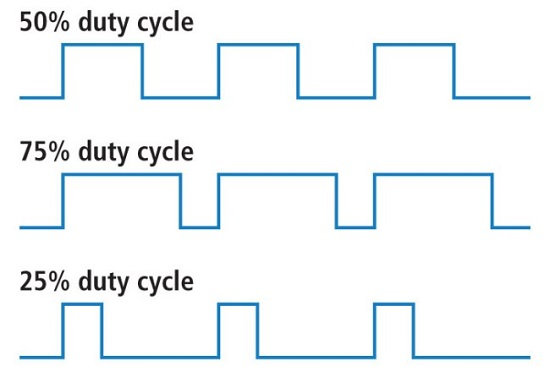
\includegraphics[height=5.5cm,width=10cm]{./Images/CH4/PWM_DutyCycle.jpg}
	\caption[چرخه کار\lr{Duty Cycle}]{چرخه کار\lr{Duty Cycle}}
	\label{چرخه کار}
	\end{figure}

\subsection{کاربرد \lr{PWM} در سروموتور}
با این قابلیت می‌توان سرعت و یا مکان ربات را کنترل کرد. که در سروموتور با توجه به وجود برد کنترلی بر روی آن قادر هستیم زاویه چرخش شفت موتور را کنترل کنیم و با این کار می‌توانیم هر پا که دارای سه لینک است را به هر جهت دلخواه حرکت دهیم چون محور دو موتور موازی هستند اما محور موتور دیگر عمود بر بقیه هست و همین باعث می‌شود محدوده زیادی را پوشش دهد.

با توجه به دیتاشیت موتور \lr{SG90}، این موتور دارای فرکانس 50 هرتز می‌باشد پس هر دوره تناوب آن برابر با 20 میلی ثانیه است. چرخه کاری این نوع موتور که در شکل \ref{SG90} آمده است، بین 1 تا 2 میلی ثانیه (در بعضی مواقع 5.0 تا 5.2 ثانیه) است که باعث می‌شود شفت از زاویه 0 تا 180 تغییر کند. به این صورت که اگر چرخه کار کمتر از 1 میلی ثانیه یا بیشتر از 2 میلی ثانیه باشد هیچ تغییری ایجاد نمی‌کند.

برای شفاف شدن این موضوع باید به این مورد اشاره کنیم که به صورت خطی بین چرخه کار 1 تا 2 میلی ثانیه (در بعضی مواقع 5.0 تا 5.2 ثانیه) و زاویه 0 تا 180 رابطه‌ای وجود دارد. به این صورت که اگر چرخه کار 1 میلی ثانیه باشد موتور در 0 درجه خود قرار دارد و اگر 5.1 میلی ثانیه باشد در 90 درجه و در نهایت اگر در 2 میلی ثانیه باشد در 180 درجه قرار دارد(شکل \ref{SG90})؛ پس ما به تمام زوایا دسترسی خواهیم داشت با توجه به این که تغییر هر زاویه تقریباً با 55.5 میکرو ثانیه معادل است.

    \begin{figure}[!h]
	\centering
	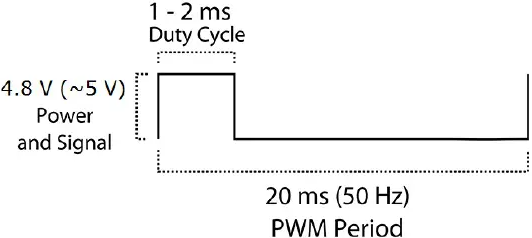
\includegraphics[height=4cm,width=6cm]{./Images/CH4/PWM_SG90_1.png}
	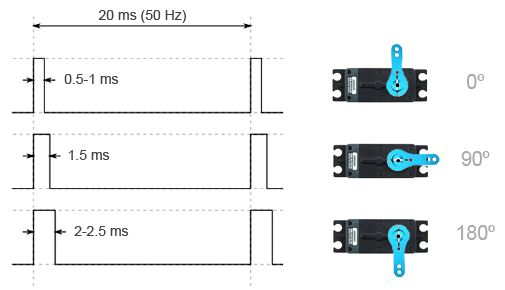
\includegraphics[height=7.6cm,width=9.2cm]{./Images/CH4/PWM_SG90_3.JPG}
	\caption[فرکانس و دوره تناوب \lr{SG90}]{فرکانس و دوره تناوب \lr{SG90}}
	\label{SG90}
	\end{figure}
	
\section{نرم‌افزار \lr{CubeMX}}
\subsection{مفهوم وکاربرد}
نرم افزار \lr{STM32CubeMX} که به اختصار به آن \lr{CubeMX} -کیوب ام ایکس- نیز می‌گویند، به جهت ساده‌تر کردن و سرعت بخشیدن به برنامه نویسی میکروکنترلرهای \lr{STM32} ایجاد شده است. ایجاد پروژه و راه‌اندازی واحدهای مختلف میکروکنترلرهای \lr{STM32} به صورت گرافیکی از جمله مهم‌ترین وظایف این نرم‌افزار است. اگرچه کارکردهای دیگری چون تخمین میزان مصرف توان میکروکنترلر را نیز دارد.

\subsection{کتابخانه‌های برنامه‌نویسی}
این نرم‌افزار، درون خود متناسب با هر میکروکنترلر شرکت  \lr{ST}، کتابخانه‌هایی چون \lr{HAL, LL, USB, TCP/IP} و ..   را دارا می‌باشد، که در صورت لزوم آن‌ها را به پروژه ما اضافه می‌کند. لایه \lr{HAL} از یک سمت با سخت‌افزار و از یک سمت با سطوح بالاتر از خود که می‌تواند \lr{Middleware} یا برنامه کاربر باشد ارتباط برقرار می‌کند. البته اگر بیان دقیق‌تر موردنظر باشد کتابخانه \lr{CMSIS} نیز باید در نظر گرفته شود که خود رابط \lr{HAL} با هسته \lr{ARM} مورد استفاده در میکروکنترلر خواهد بود.

این نرم‌افزار علاوه بر فراهم کردن محیط تصویری و قابلیت فعال کردن و انجام اکثر تنظیمات به صورت گرافیکی این امکان را می‌دهد که کاربر یک دید کلی نسبت به میکروکنترلر خود داشته باشد و مناسب‌ترین میکروکنترلر برای کار خود را انتخاب کند.

\newpage
با استفاده از این نرم افزار کتابخانه های \lr{HAL} و \lr{LL} به طور خودکار و بسته به انتخاب هایی که انجام شده باشد به کد اضافه می‌شود. همچنین مقداردهی‌های اولیه و بعضی از تنظیمات به صورت خودکار انجام می‌شود.
\begin{itemize}
	\item \textbf{توابع \lr{(Low Layer)LL}}: در این روش دیگر به‌صورت مستقیم با رجیسترها کار نمی‌شود و فقط از توابعی به نام توابع \lr{LL} استفاده خواهد شد که خود این توابع با توجه به آرگومان‌های ورودی‌شان، رجیسترها را مقداردهی می‌کنند. با فراخوانی هرکدام از این توابع عملاً بخشی از یک واحد جانبی راه‌اندازی می‌شود. برای اینکه یک واحد جانبی به‌طور کامل راه‌اندازی شود باید از یک توالی خاص از چندین توابع \lr{LL} استفاده شود.
	
	\item \textbf{توابع \lr{(Hardware Abstraction Layer)HAL}}: در این نوع توابع که در بالاترین سطح ممکن است، با سطح رجیستر خیلی فاصله‌ وجود دارد و عملاً به‌ندرت از رجیسترها استفاده می‌شود، اگرچه دسترسی به رجییسترها در این سطح بدون هیچ مشکلی ممکن است و با استفاده از ماکروهایی می‌توان به رجیسترها دسترسی داشت. وقتی‌که از یک تابع \lr{HAL} استفاده می‌شود علاوه بر اینکه خودش رجیسترهای یک بخش را تنظیم می‌کند، در اکثر موارد بسیاری از کارهایی که در توابع \lr{LL} باید خود کاربر انجام می‌داد را نیز انجام می‌دهد.
	
	مثلاً اگر قرار بود در توابع \lr{LL}، از 5 تابع استفاده شود و کمی هم توابع زبان \lr{C} به‌کار برده شود تا یک واحد جانبی راه‌اندازی شود، ممکن است تمامی این کارها با یک تابع \lr{HAL} انجام شود.
	\item \textbf{توابع \lr{(Standard peripheral libraries)SPL}}: توابع \lr{SPL} در سطح میانی قرار دارند و می‌توان گفت سطحی بین \lr{LL} و \lr{HAL} را دارا هستند. البته این توابع دیگر به‌روزرسانی نمی‌شوند. بنابراین امروزه به جای این توابع از توابع \lr{HAL} که قابلیت‌های بسیار بهتری دارند، استفاده می‌شود.
	
\end{itemize}

توابع \lr{HAL} به‌قدری همه‌چیز را آماده کرده‌اند که اگر به خوبی بررسی شوند، مشاهده می‌شود که در بعضی موارد اگر کاربر سهواً یا از روی ندانستن اشتباهی انجام داده باشد، آن اشتباه را اگر ممکن باشد و تشخیص بدهد، تصحیح می‌کند. منطقاً هرکدام از این روش‌ها برای هدف خاصی مناسب هستند، و این‌گونه نیست که یک روش کاملاً ناکارآمد و به‌دردنخور باشد. به‌عنوان‌مثال اگر هدف سرعت برنامه باشد، توابع \lr{HAL} اصلاً توصیه نمی‌شوند و رجیستری بهترین انتخاب است. در نقطه‌ی مقابل اگر هدف سرعت توسعه‌ی پروژه باشد و سرعت برنامه مدنظر نباشد، بهترین انتخاب توابع \lr{HAL} هستند و رجیستری اصلاً توصیه نمی‌شود.
\newpage
\subsection{کانفیگ پایه‌های میکروکنترلر}
هر پین میکروکنترلر ممکن است چندین گزینه برای کانفیگ شدن داشته باشد.  برای مثال اگر به دیتاشیت \lr{STMF103C8T6} مراجعه کنید. برای پین \lr{PB6} چندین کارکرد از جمله \lr{USART1-TX} و \lr{I2C1-SCL} و \lr{Timer4-Channel1} وجود دارد که تنها باید یکی از آنها را انتخاب نمود. ما نمی‌توانیم این پایه را هم به عنوان \lr{Tx} واحد \lr{USART1} و هم به عنوان \lr{SCL} پروتکل \lr{I2C} تنظیم کنیم. چراکه این کار باعث به وجود آمدن تداخل می‌شود. از ویژگی‌های مفید \lr{CubeMX} این است که در صورت امکان تداخل در کانفیگ پین‎های میکروکنترلر، این موضوع را به ما نشان می‌دهد و مانع از بروز مشکل می‌شود.

    \begin{figure}[!h]
	\centering
	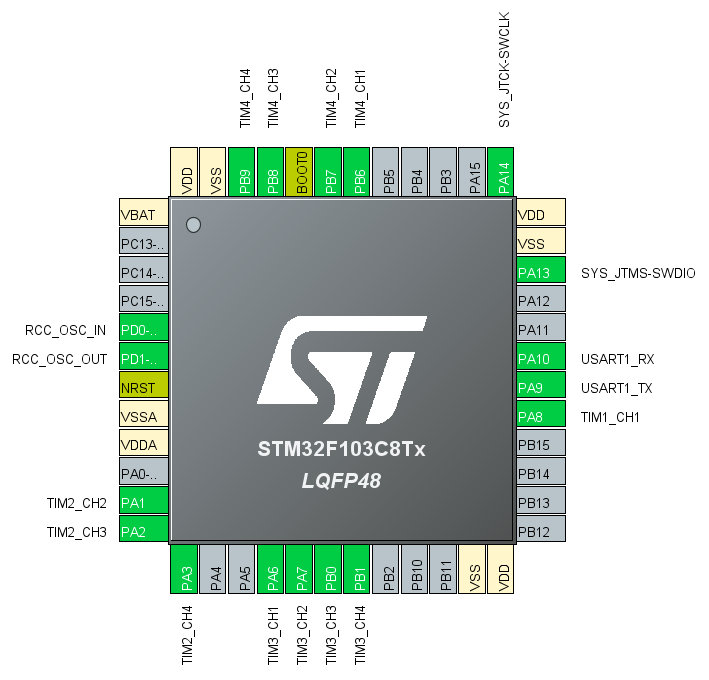
\includegraphics[height=8cm,width=8cm]{./Images/CH4/CubeMX_2.PNG}
	\caption[کانفیگ میکروکنترلر]{کانفیگ میکروکنترلر}
	\label{کانفیگ میکروکنترلر}
	\end{figure}

\subsection{تنظیم کلاک}
به نوعی مشابه ویژگی قبلی، در قسمت تنظیم کلاک نرم‌افزار \lr{CubeMX} امکانی وجود دارد که کمک می‌کند به تنظیم قسمت‌های مختلف کلاک  پرداخته شود. در واقع در اینجا هم اگر مقداری خارج از حد مجاز به قسمتی از کلاک داده شود، با رنگ قرمز وجود مشکل را اعلام می‌کند. در صورت به وجود آمدن این وضعیت، به صورت اتوماتیک (توسط نرم افزار) یا دستی (توسط خودمان) مقادیر به حالت مجاز تغییر داده می‌شوند.

    \begin{figure}[!h]
	\centering
	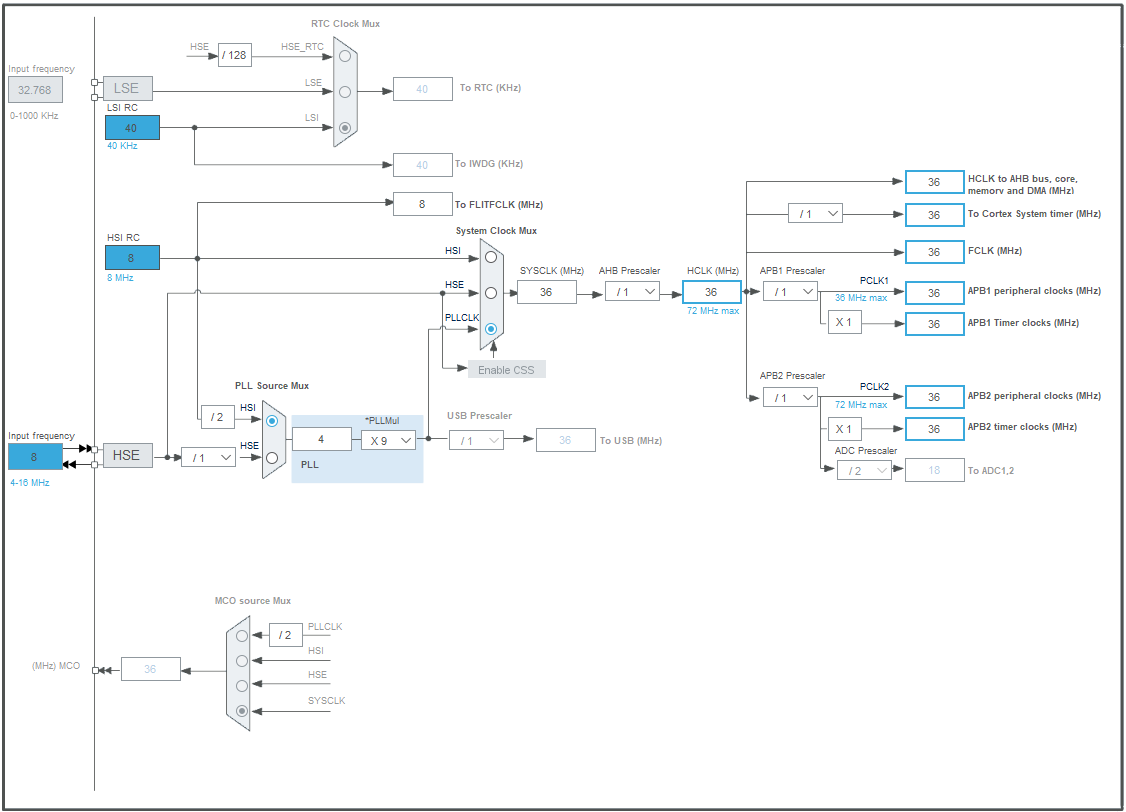
\includegraphics[height=7cm,width=12cm]{./Images/CH4/CubeMX_1.PNG}
	\caption[تنظیم کلاک]{تنظیم کلاک}
	\label{تنظیم کلاک}
	\end{figure}

\vspace{1cm}
\subsection{تنظیمات موردنیاز برای ربات چهارپا}
کلاک داخلی میکروکنترلر 8 مگاهرتز می‌باشد و با استفاده از کریستال خارجی می‌توان به 72 مگاهرتز ارتقا داد، در این پروژه هم برای سرعت بالاتر از کریستال خارجی استفاده شده است و به این دلیل که به سرعت خیلی بالایی نیاز نیست ولی دقت پارامتر مهمی است پس کلاک را روی 36 مگاهرتز تنظیم شده است.

در این پروژه همان‌طورکه قبلا به آن اشاره شده است، به 12 پایه \lr{PWM} نیاز است و در میکروکنترلر مورد استفاده چهار تایمر وجود دارد که هر تایمر دارای 4 کانال می‌باشد پس، از 12 تا از این کانال‌ها استفاده می‌شود. برای درست کار کردن هر تایمر در ابتدا نیاز است که تنظیماتی اعمال شود.

همانطور که در فصل قبل به آن اشاره شد، سروموتور به دامنه زمانی 20 میلی ثانیه یا فرکانس 50 هرتز نیاز دارد. در این نرم‌افزار با دو پارامتر می‌توان به مقدار مطلوب رسید که فرمول به شکل زیر است:
\begin{equation}
	F_{PWM} = \frac{F_{CLK}}{(ARR + 1)*(PSC + 1)}
\end{equation}

پارامترهای \lr{PSC}\unskip\LTRfootnote{Prescale} و \lr{ARR}\unskip\LTRfootnote{Auto Reload Register}(\lr{counter period}) به شکلی انتخاب می‌شوند تا به فرکانس 50 هرتز دست یافته شود. فرکانس کلاک برابر با 36 مگاهرتز است پس مخرج که ضرب دوتا پارامتر می‌باشد باید برابر با 720000 شود؛ حال می‌توان هر مقداری برای این دو پارامتر درنظر گرفت ولی با توجه به چرخه کار مدنظر برای \lr{PSC} مقداری خاص انتخاب می‌شود. 
\begin{equation}
	DutyCycle =\frac{CCR}{ARR}
\end{equation}
نیاز است ابتدا و انتهای بازه برای مقداردهی \lr{PWM} بدست آورده شود که مقداردهی آن به صورت رجیستری است:
\begin{itemize}
	\item \textbf{زاویه 0 درجه}: همانطور که گفته شد بین بازه 5.0 تا 1 میلی ثانیه سیگنال روشن است پس نسبت چرخه کار 5.2 درصد می‌باشد و برای راحتی در محاسبات، \lr{PSC} 999 در نظر گرفته می‌شود، درنهایت مقدار \lr{CCR} 25 بدست می‌آید.
	\item \textbf{زاویه 90 درجه}: برای میانه بازه، نسبت چرخه کار 5.1 به 20 می‌باشد که برابر با 7.5 درصد است و همانطورکه \lr{PSC} 999 قرار داده شده است پس \lr{CCR} باید 75 مقداری دهی شود.
	\item \textbf{زاویه 180 درجه}: در نهایت، برای بیشترین زاویه که 180 درجه می‌باشد، سیگنال به اندازه 2 تا 5.2 میلی ثانیه روشن می‌ماند پس نسبت چرخه کار برابر با 5.12 می‌شود و مقدار انتهایی \lr{CCR} هم 125 می‌باشد. 
\end{itemize}

    \begin{figure}[!h]
	\centering
	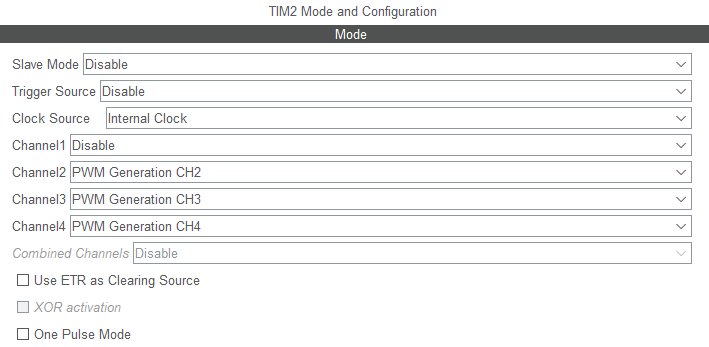
\includegraphics[height=6.5cm,width=12cm]{./Images/CH4/CubeMX_PWM_Config_1.PNG}
	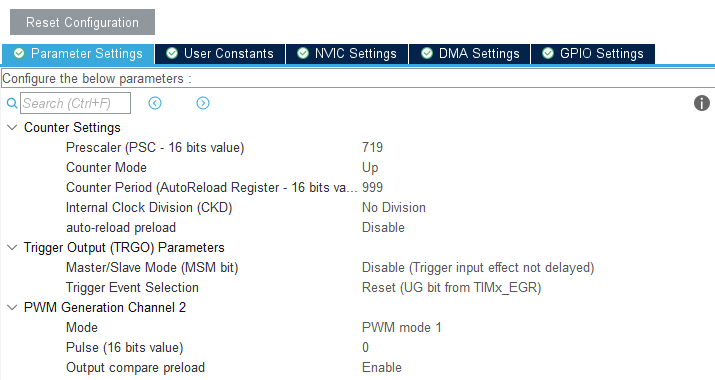
\includegraphics[height=7cm,width=12cm]{./Images/CH4/CubeMX_PWM_Config_2.PNG}
	\caption[تنظیمات تایمر]{تنظیمات تایمر}
	\label{تنظیمات تایمر}
	\end{figure}

برای تنظیمات پروتکل \lr{UART} هم در ابتدا باید \lr{Baud Rate} یکسانی برای دو پردازنده انتخاب شود تا با سرعت یکسانی کار کنند که در این پروژه بر روی 115200 بیت بر ثانیه تنظیم شده است. سپس در قسمت انتخاب مد، گزینه آسنکرون انتخاب شده است به این دلیل که به همزمانی نیاز نیست و همچنین حجم داده ارسالی خیلی زیادی وجود ندارد و سرعت انتقال داده این مد مناسب است و به سرعت بالاتری که منجر به استفاده از ارتباط سنکرون شود نیازی نیست.

دو نکته دیگر در کار با ارتباط سریال خیلی مهم هستند؛ زمانی که دوریبین مانعی را تشخیص دهد از طریق سریال به پردازنده اصلی داده‌ای ارسال می‌شود که کدام نوع مانع دیده شده است، چالشی که با آن مواجه شدیم این بود که ما نیاز به ارسال بلادرنگ\LTRfootnote{Real Time} داده است اما در سمت دریافت، داده فقط یکبار دریافت می‌شود پس ما مد گیرنده را روی \lr{Circular} قرار می‌دهیم که در هرلحظه داده را بگیرد.

در نهایت هم برای بهینه شدن کد و عملکرد آن، که در هر لحظه قصد خواندن داده نداشته باشد از وقفه\LTRfootnote{Interrupt} استفاده شده است که باعث می‌شود همان لحظه که داده فرستاده می‌شود، داده را خوانده و آن را ذخیره کند.

    \begin{figure}[!h]
	\centering
	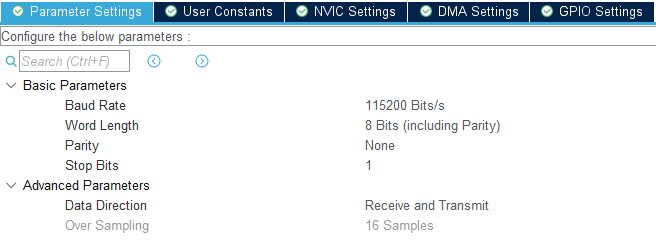
\includegraphics[height=3.5cm,width=12cm]{./Images/CH4/CubeMX_UART_Config_1.PNG}
	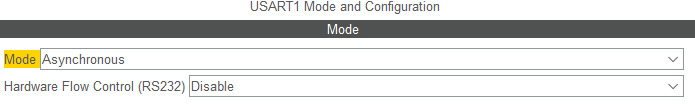
\includegraphics[height=1.5cm,width=12cm]{./Images/CH4/CubeMX_UART_Config_4.PNG}
	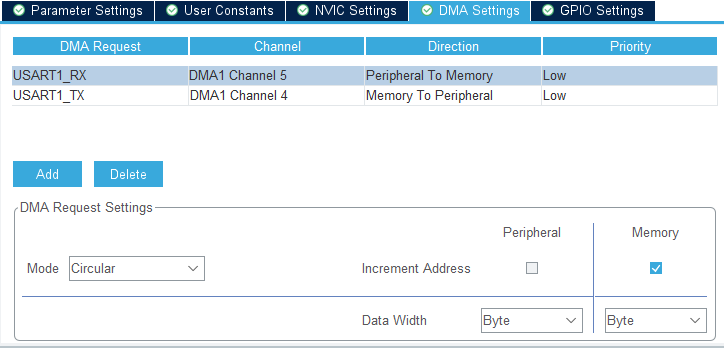
\includegraphics[height=4.5cm,width=12cm]{./Images/CH4/CubeMX_UART_Config_3.PNG}
	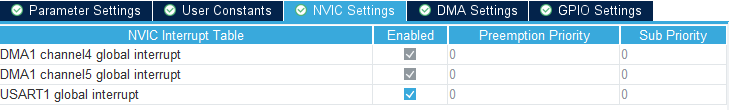
\includegraphics[height=2cm,width=12cm]{./Images/CH4/CubeMX_UART_Config_2.PNG}
	\caption[تنظیمات ارتباط سریال]{تنظیمات ارتباط سریال}
	\label{تنظیمات ارتباط سریال}
	\end{figure}

\section{برنامه‌نویسی در نرم‌افزار \lr{Keil}}
\subsection{نرم‌افزار \lr{Keil} چیست؟}
نرم افزار \lr{Keil} یا \lr{Keil MDK} یا \lr{MDK} (مخفف \lr{Microcontroller Development Kit}) که ساخت شرکت \lr{Keil} است، برای توسعۀ طیف وسیعی از میکروکنترلرهای \lr{ARM Cortex-M } و میکروکنترلرهای دیگر است. این نرم افزار شامل یک \lr{IDE} است که \lr{µVision IDE} نام دارد. همچنین شامل محیط ویرایشگر کد، پروگرامر و دیباگر، شبیه ساز، کامپایلر و \lr{…} است و این امکان را به کاربر می دهد که به راحتی بتواند برای میکروکنترلرها برنامه نویسی کند.

در ابتدا تنظیمات موردنیاز را در \lr{Cube MX} انجام می‌دهیم و برای ما در \lr{Keil} کد خام تولید می‌کند تا دیگر نیاز نباشد تمام کد را از ابتدا بنویسیم.
\subsection{تنظیم تایمرها}
ما در ربات 12 عدد موتور داریم که هر موتور با \lr{PWM} کار می‌کند پس نیاز به 12 پایه تایمر داریم. همانطور که در قسمت‌های قبل به آن شاره شد در این میکروکنترلر 4 عدد تایمر داریم که هر تایمر هم 4 عدد کانال دارد پس در کل 16 پایه با این قابلیت موجود است. به این دلیل که هر پایه در این میکروکنترلر چندین قابلیت دارد باید حتما به آن دستور داده شود که از کدام قبلیت می‌خواهیم استفاده کنیم تا تصادفاً مشکلی پیش نیاید. هیچ تفاوتی وجود ندارد که از کدام 16 پایه استفاده کنیم؛ فقط دو تا از پایه‌ها برای ارتباط سریال استفاده می‌شوند پس انتخاب از 14 پایه دیگر است.
\begin{latin}
	\lstinputlisting[style=c_style]{code/Timer_Initialize.c}
\end{latin}
\subsection{تابع حرکت موتور}
در مرحله بعدی که تایمر را فعالسازی کردیم، توابع حرکت موتورها را می‌نویسیم. برای حرکت دادن هر موتور نیاز داریم که به صورت رجیستری به آن دستور بدهیم و همانطور که قبلاً به آن اشاره کردیم، مجاز هستیم در بازه 25 تا 125 فرمان بدهیم. برای انجام اینکار نیاز داریم که شماره تایمر، کانال و مقدار \lr{PWM} را بدانیم. نکته مهم آن است که ما مقدار در لحظه هر موتور را در یک آرایه ذخیره می‌کنیم و این تابع دستور می‌دهیم که از زاویه قبلی به زاویه جدید و دلخواه برود. 
\begin{latin}
	\lstinputlisting[style=c_style]{code/Move.c}
\end{latin}
نوعی دیگر از حرکت که برای موتورها درنظر گرفتیم، حرکت چهارپا همزمان است. به این صورت که چهارپای اول، دوم یا سوم به صورت همزمان حرکت می‌‌کنند که برای بلند شدن ربات استفاده می‌شود چون اگر هر پا مجزا حرکت بکنند ربات تعادل نخواهد داشت و ربات به یک سمت می‌افتد.
\begin{latin}
	\lstinputlisting[style=c_style]{code/Move_All_Motors.c}
\end{latin}
\subsection{چهار حرکت اصلی ربات}
بعد از آنکه تمام حرکت‌ها را نوشتیم و بدست آوردیم شروع به نوشتن چهار حرکت اصلی می‌کنیم اما قبل از آن باید دستوری به ربات بدهیم که در ابتدا که شروع به حرکت می‌کند، به یک نقطه یا حالت اولیه برود که تعادل داشته باشد و به راحتی بدون لغزش بایستد.

در این تابع ابتدا به چهار موتور اول هر پا سپس چهار موتور دوم و در انتها هم به چهار موتور سوم دستور می‌دهیم که به زاویه مطلوب برود. به اینصورت عمل می‌کند که تمام چهار موتور با یکدیگر حرکت می‌کنند و برای اینکار تابع \lr{Move All} را فراخوانی می‌کنیم.

\begin{latin}
	\lstinputlisting[style=c_style]{code/Home.c}
\end{latin}

حرکت بعدی که آن را پیاده سازی کردیم، حرکت به سمت جلو می‌باشد که ربات با کمک اصطکاک و لغزش به سمت جلو حرکت می‌کند. در این حرکت ابتدا یکی از دو پای جلو باز شده تا مرکز ثقل به آن سمت برود و در این حالت پای مقابل آن در عقب ربات می‌تواند از زمین بلند شود و به سمت جلو برود و سپس پای جلو ربات که باز شده بود به حالت قبلی برمی‌گردد اما پای عقب جلو تر از حالت اولیه و صفر خود است پس وقتی به حالت قبلی برمی‌گردد، ربات به کمک اصطکاک پا به جلو حرکت می‌کند.

\begin{latin}
	\lstinputlisting[style=c_style]{code/Forward.c}
\end{latin}

حرکت به سمت عقب رفتن هم به همین شکل است فقط پاهای جلو و عقب عکس جلو رفتن عمل می‌کنند. ابتدا پای عقب باز شده و سپس پای مقابل آن در جلو ربات ابتدا از زمین بلند شده و به سمت عقب حرکت می‌کند؛ سپس پای عقب به حالت اولیه باز می‌گردد و پای جلو که به زمین رسیده است به سمت جلو حرکت می‌کند و با اصطکاک ایجاد شده ربات به سمت عقب می‌رود.

\begin{latin}
	\lstinputlisting[style=c_style]{code/Backward.c}
\end{latin}

در نهایت هم چرخش به سمت چپ و راست را داریم که به این صورت است که برای چرخش به چپ پای عقب راست باز شده تا پای جلو چپ از زمین جدا شده به سمت عقب حرکت کند و سپس بسته شده تا پای جلو چپ به زمین برسد؛ بعد از آن همان پا بسته می‌شود تا پای عقب راست از زمین جدا شده و جلو برود. در نهایت با برگشتن پای جلو چپ به حالت قبلی، دو پا همزمان به حالت اولیه حرکت می‌کنند و ربات به سمت چپ می‌چرخد.

\begin{latin}
	\lstinputlisting[style=c_style]{code/Turn_Left.c}
\end{latin}

\vspace{1cm}
برای چرخش به راست هم به همین شکل فقط به جای پای عقب راست و جلو چپ، پای عقب چپ و جلو راست را داریم.

\begin{latin}
	\lstinputlisting[style=c_style]{code/Turn_Right.c}
\end{latin}

\subsection{عملکرد کلی ربات}
با همه نکاتی که گفتیم و توابعی که نوشتیم باید از آن‌‌ها استفاده کنیم به شکلی که ربات به سمت هدف حرکت کرده و از موانع دور شود. پس با استفاده از دوربین و تشخیص رنگ یک کاراکتر از طریق ارتباط سریال دریافت می‌کنیم و نسبت به رنگی که دارد دستور می‌دهیم که چه کاری انجام شود. ما کنار کاراکتر رنگ یک عدد سه رقمی از مساحت مانع هم می‌گیریم که هرچه به مانع نزدیکتر شویم این عدد بزرگتر شده پس می‌دانیم کی باید حرکت دیگری انجام دهیم که برخورد نداشته باشیم.

\begin{latin}
	\lstinputlisting[style=c_style]{code/Main.c}
\end{latin}